














\section{Montagesystem}
%\begin{comment}
    

\subsection{Befestigung am Gebäude}
\subsubsection{Dachhaken}
Für Ziegeldächer\\
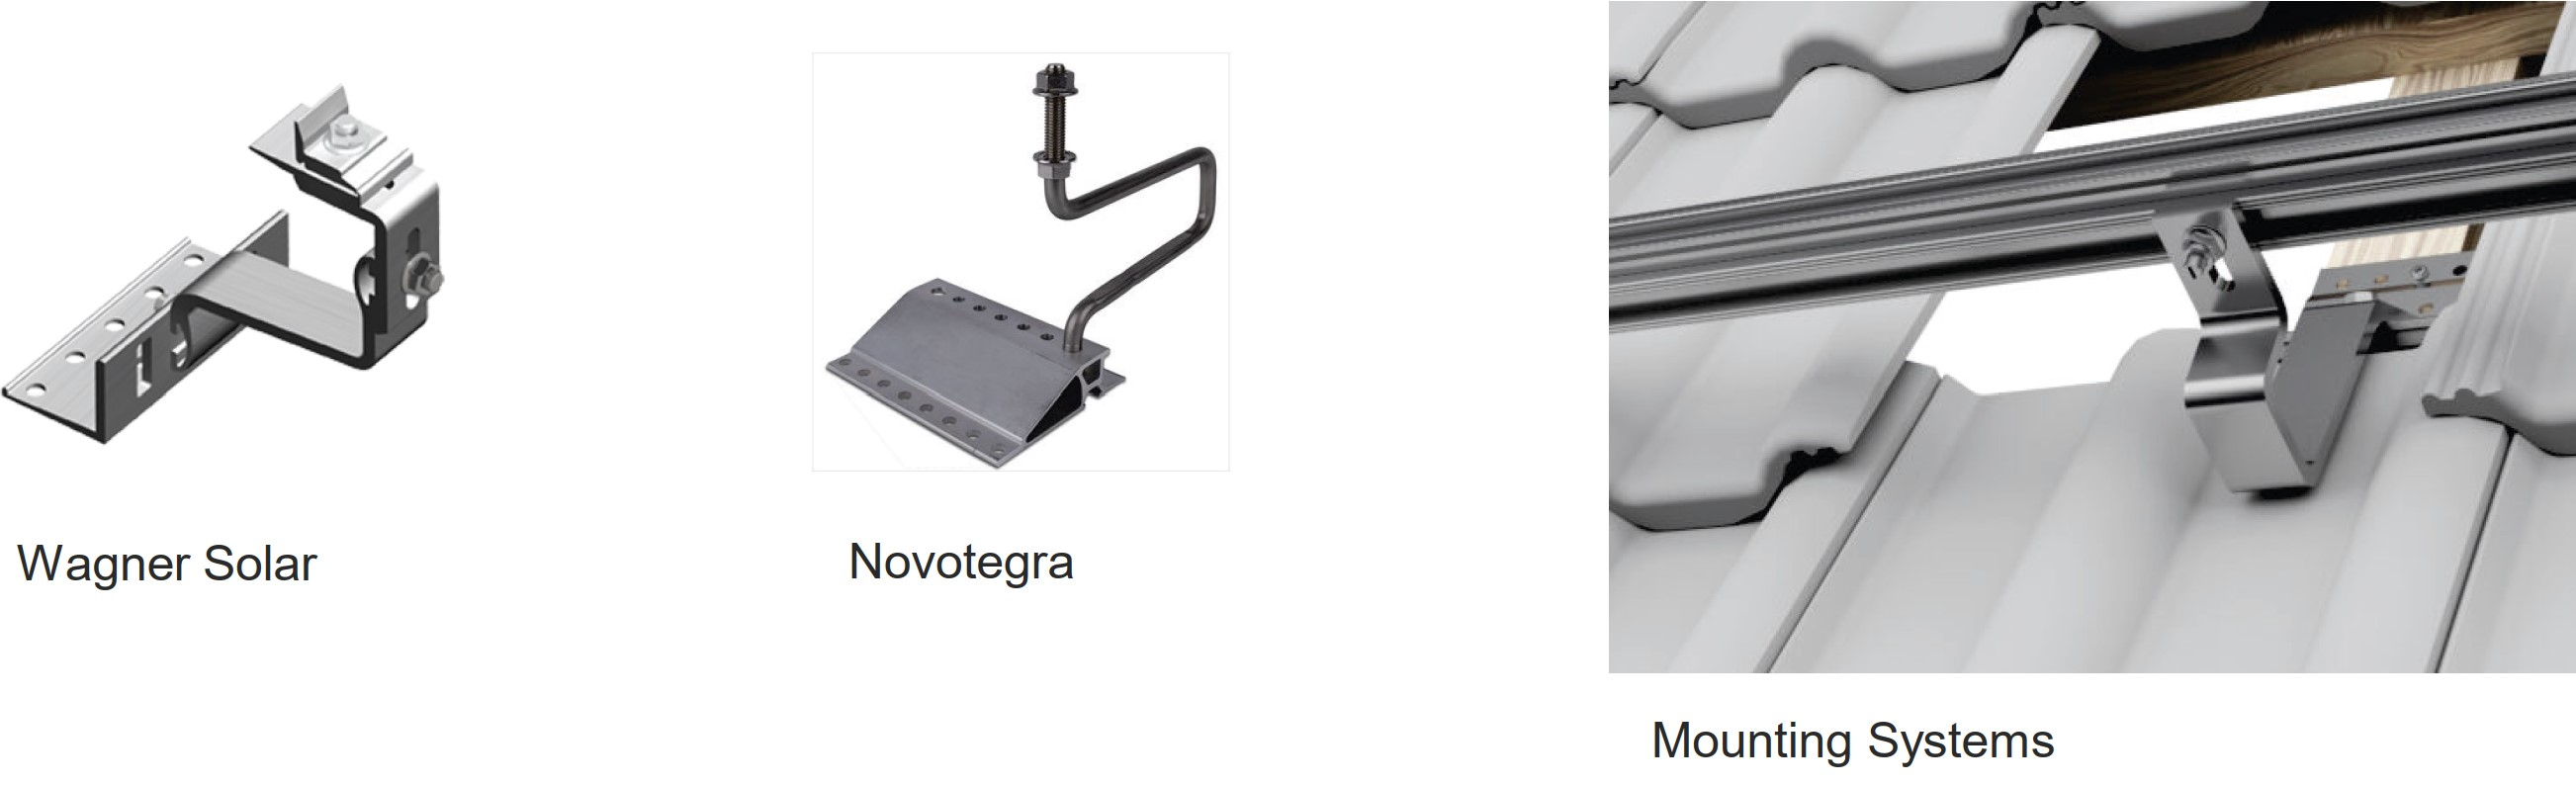
\includegraphics[width=0.95\columnwidth]{images/Dachhaken.jpg}


\subsubsection{Stockschrauben}
Für Well- und Trapezblech-, Faserzement- und Sandwichdächer\\
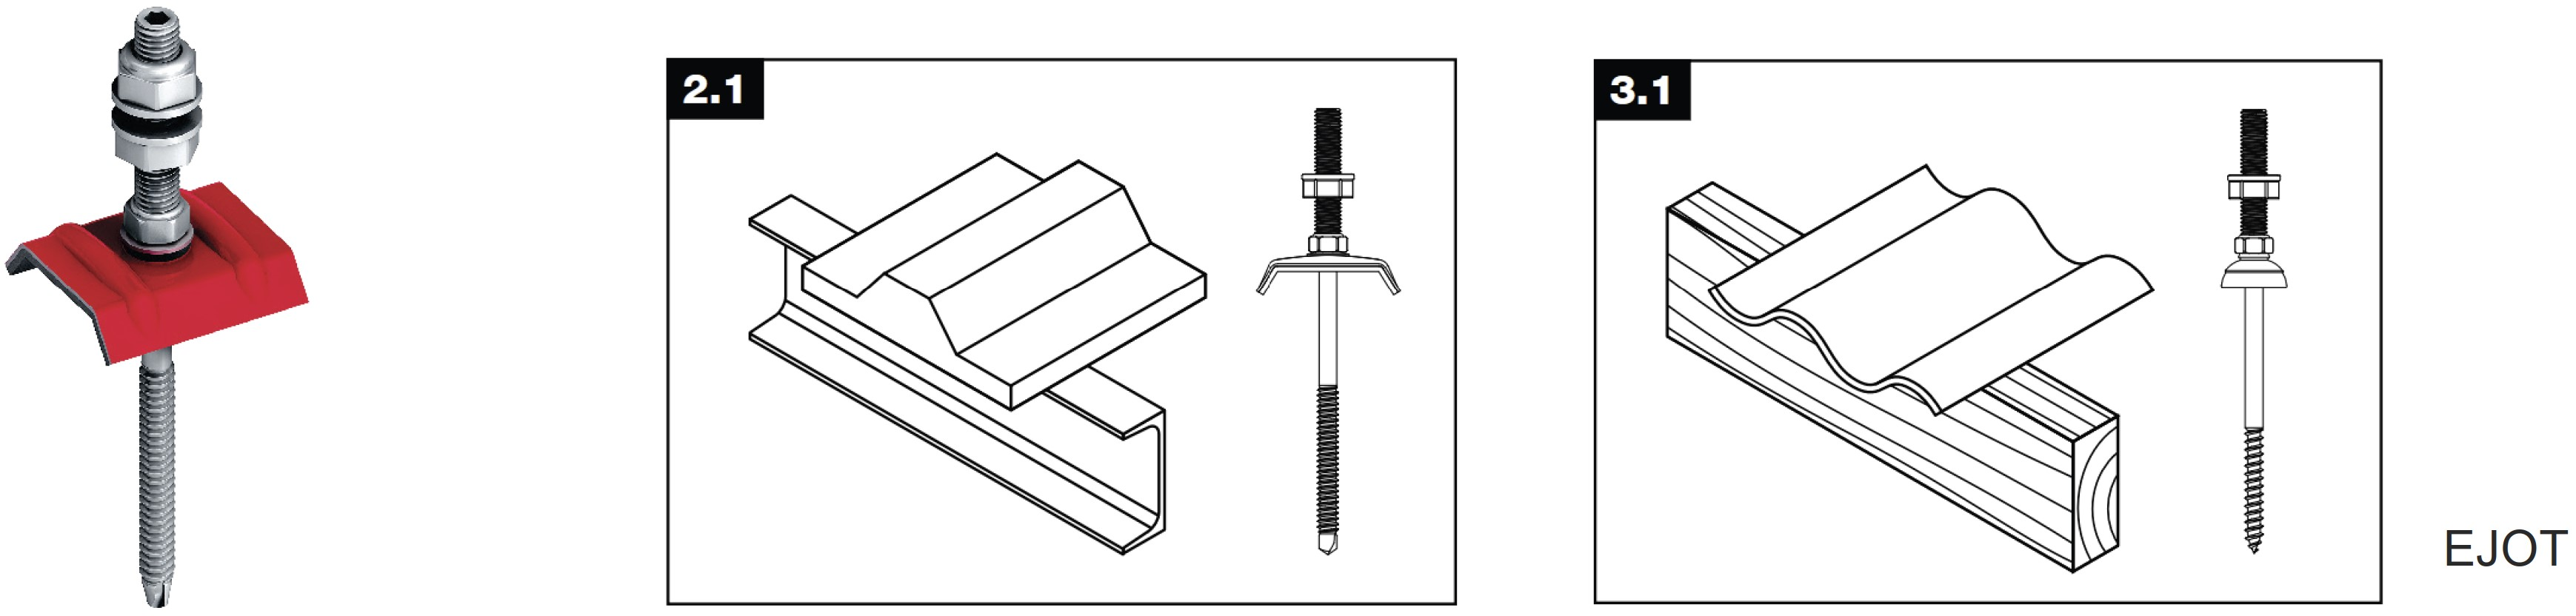
\includegraphics[width=0.95\columnwidth]{images/Stockschrauben.jpg}


\subsubsection{Stehfalzklemmen}
Für Stehfalzdächer\\
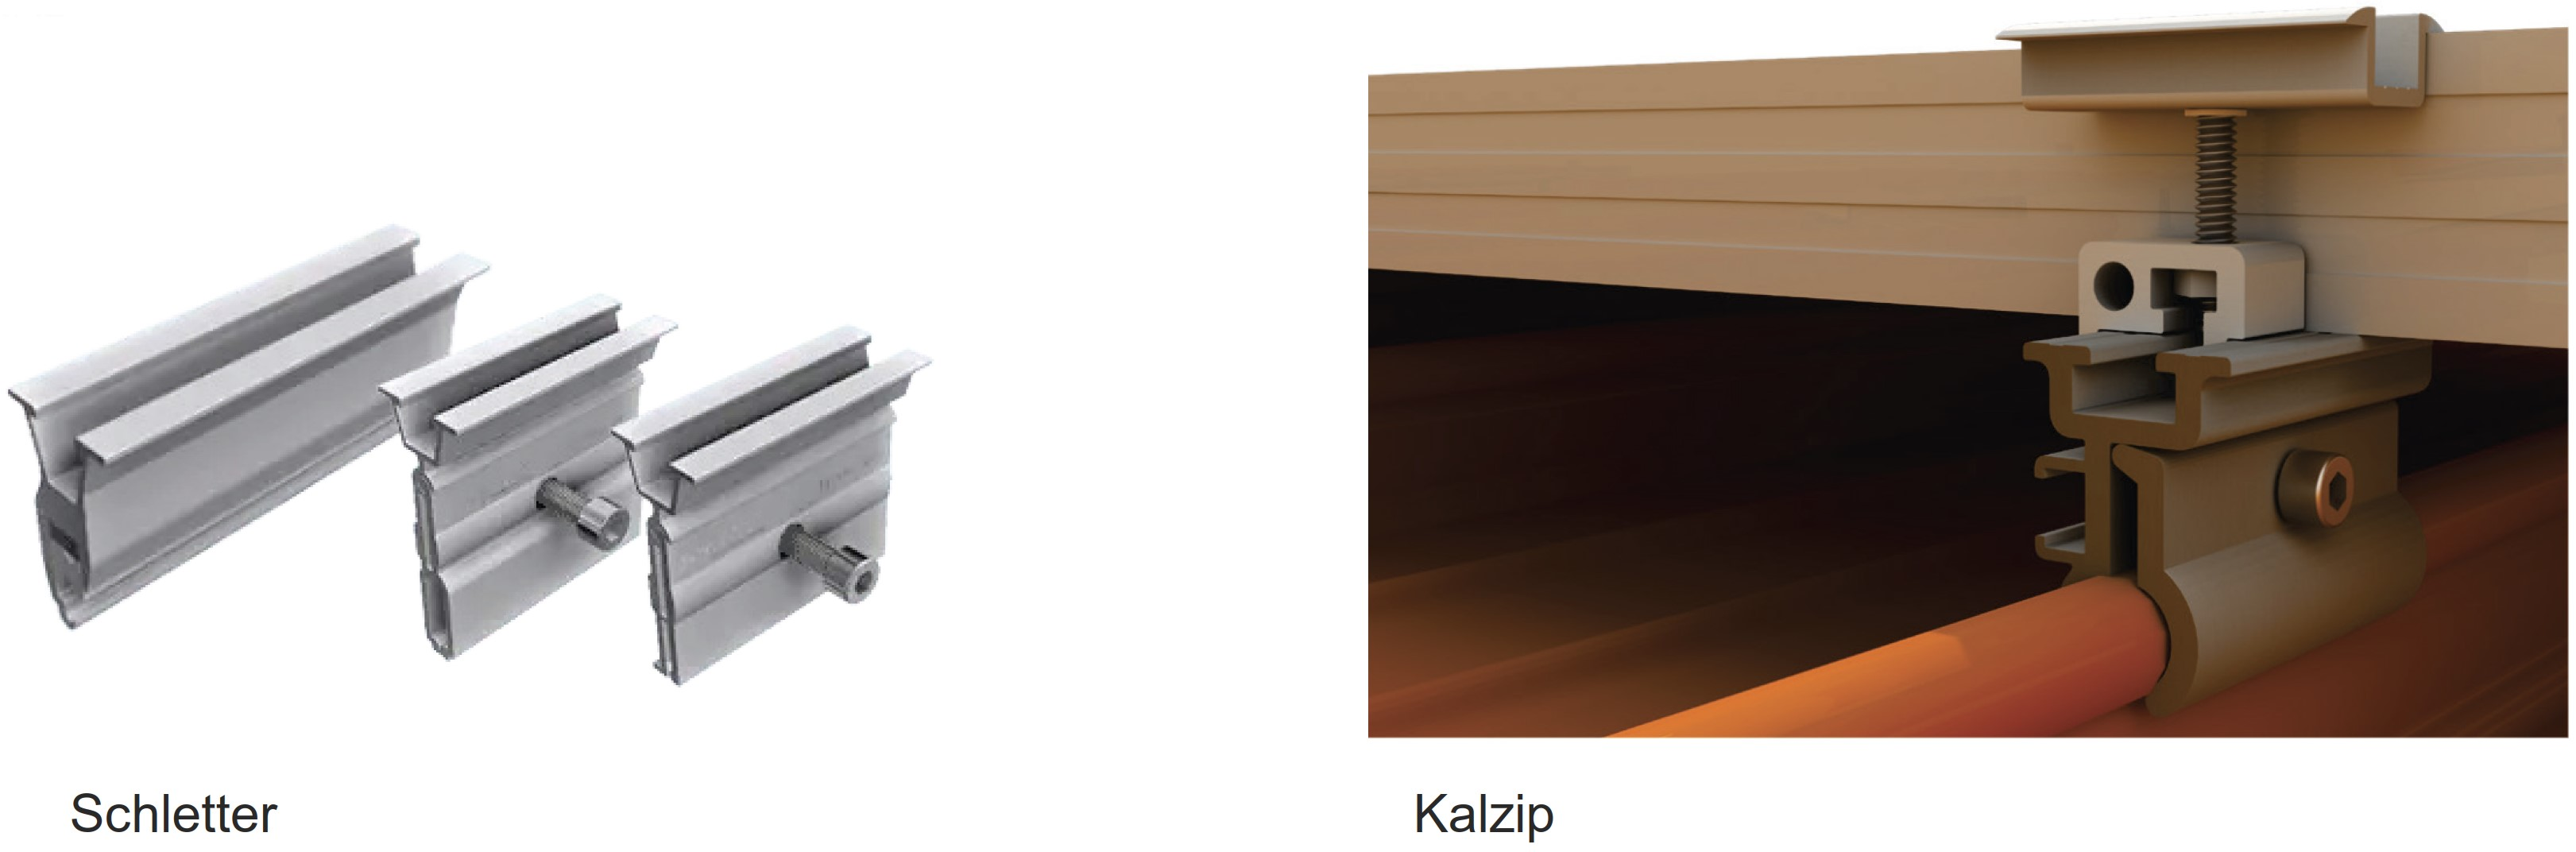
\includegraphics[width=0.95\columnwidth]{images/Stehfalzklemmen.jpg}


\subsubsection{Nieten, Blechschrauben}
Für Trapezblechdächer\\
\begin{minipage}[t]{0.48\columnwidth}
    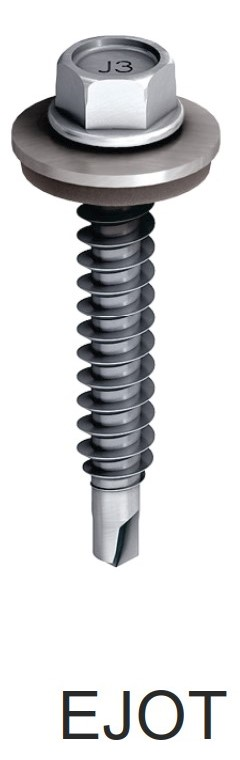
\includegraphics[width=0.15\columnwidth]{images/Nieten_Blechschrauben_1.jpg}
\end{minipage}
\hfill
\begin{minipage}[t]{0.48\columnwidth}
    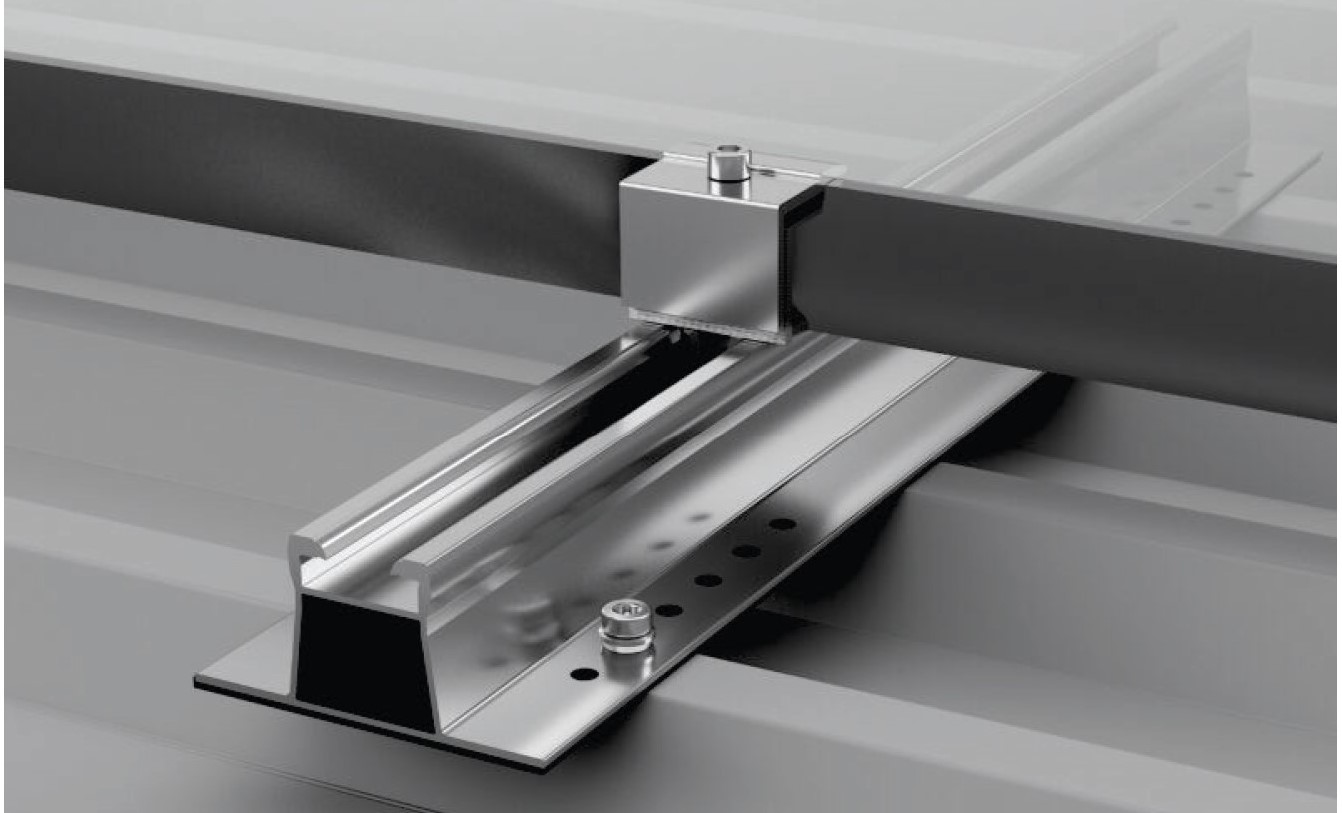
\includegraphics[width=0.85\columnwidth]{images/Nieten_Blechschrauben_2.jpg}
\end{minipage}



\subsection{Tragkonstruktion / Schienensystem}

\subsubsection{Einlagiges Schienensystem}

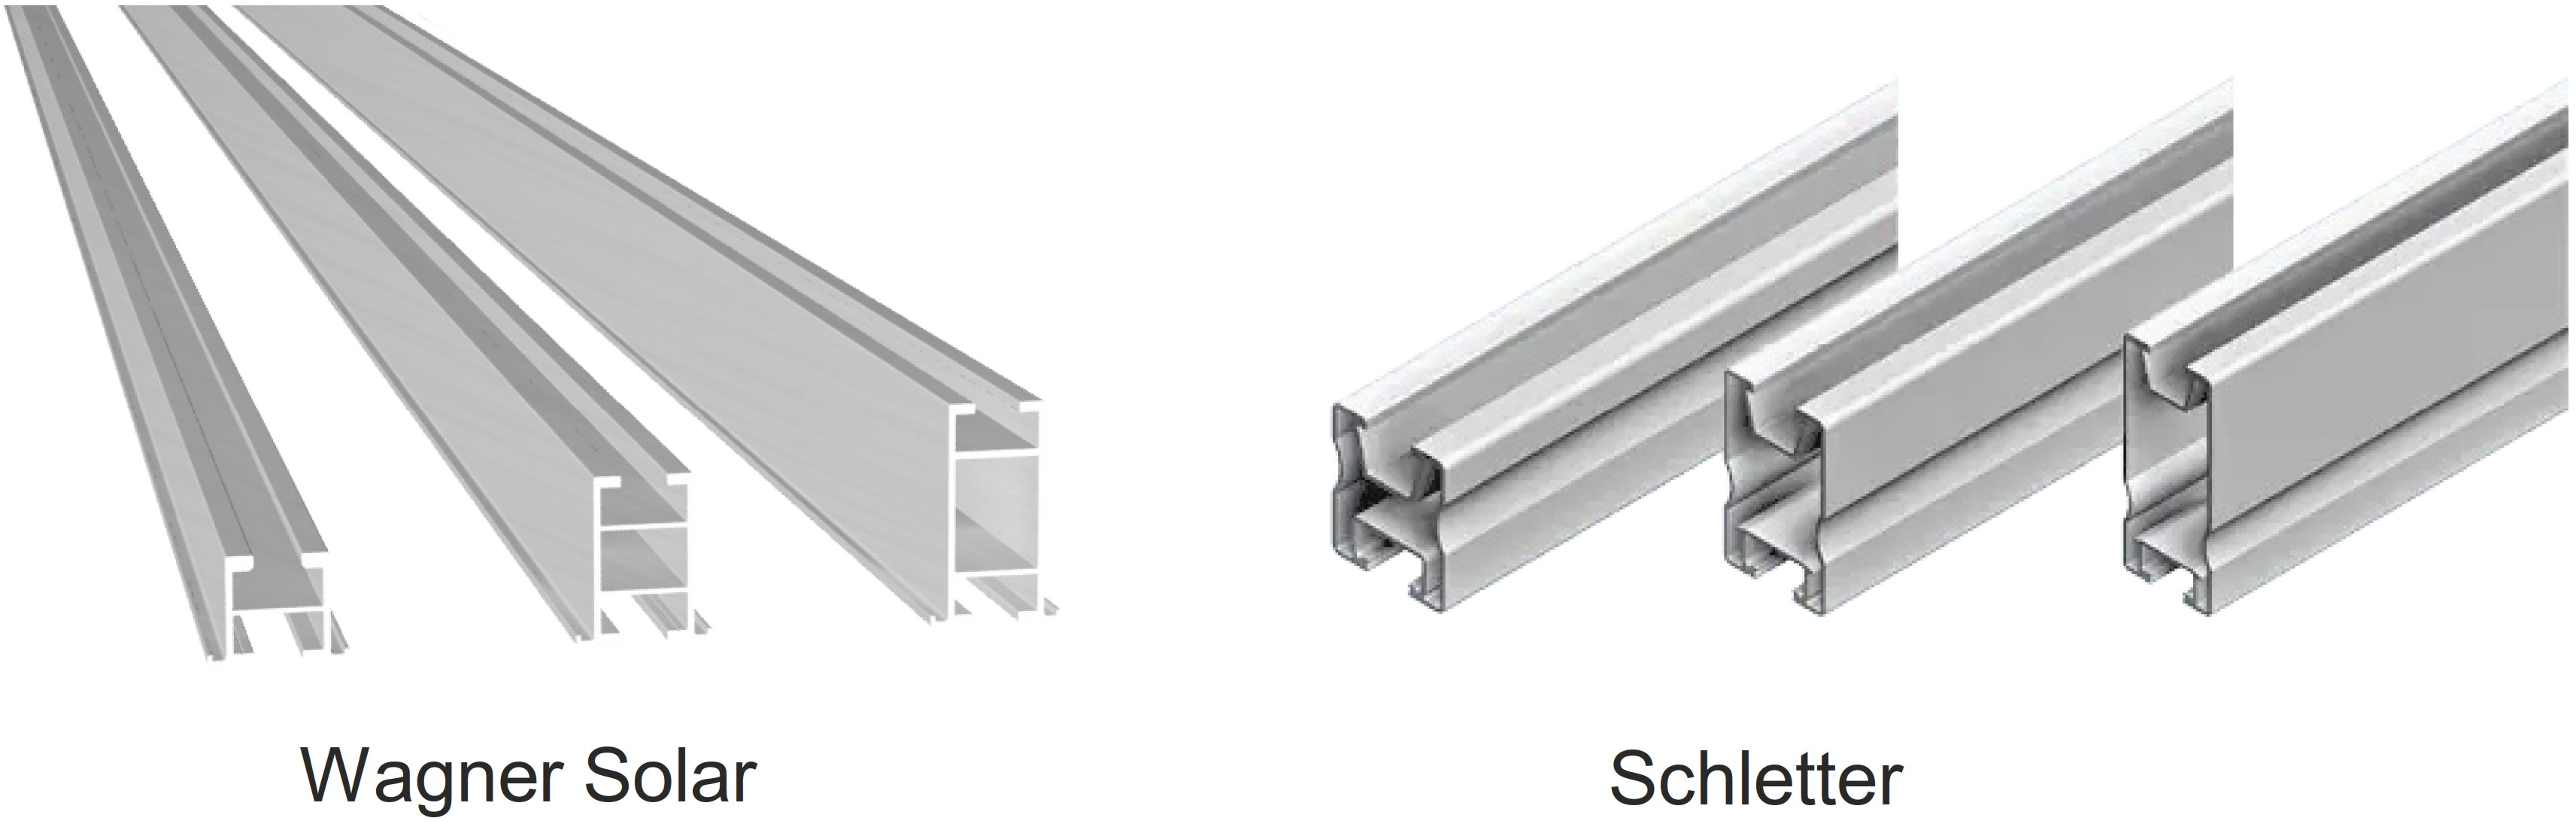
\includegraphics[width=0.85\columnwidth]{images/Einlagiges Schienensystem 1.jpg}\\

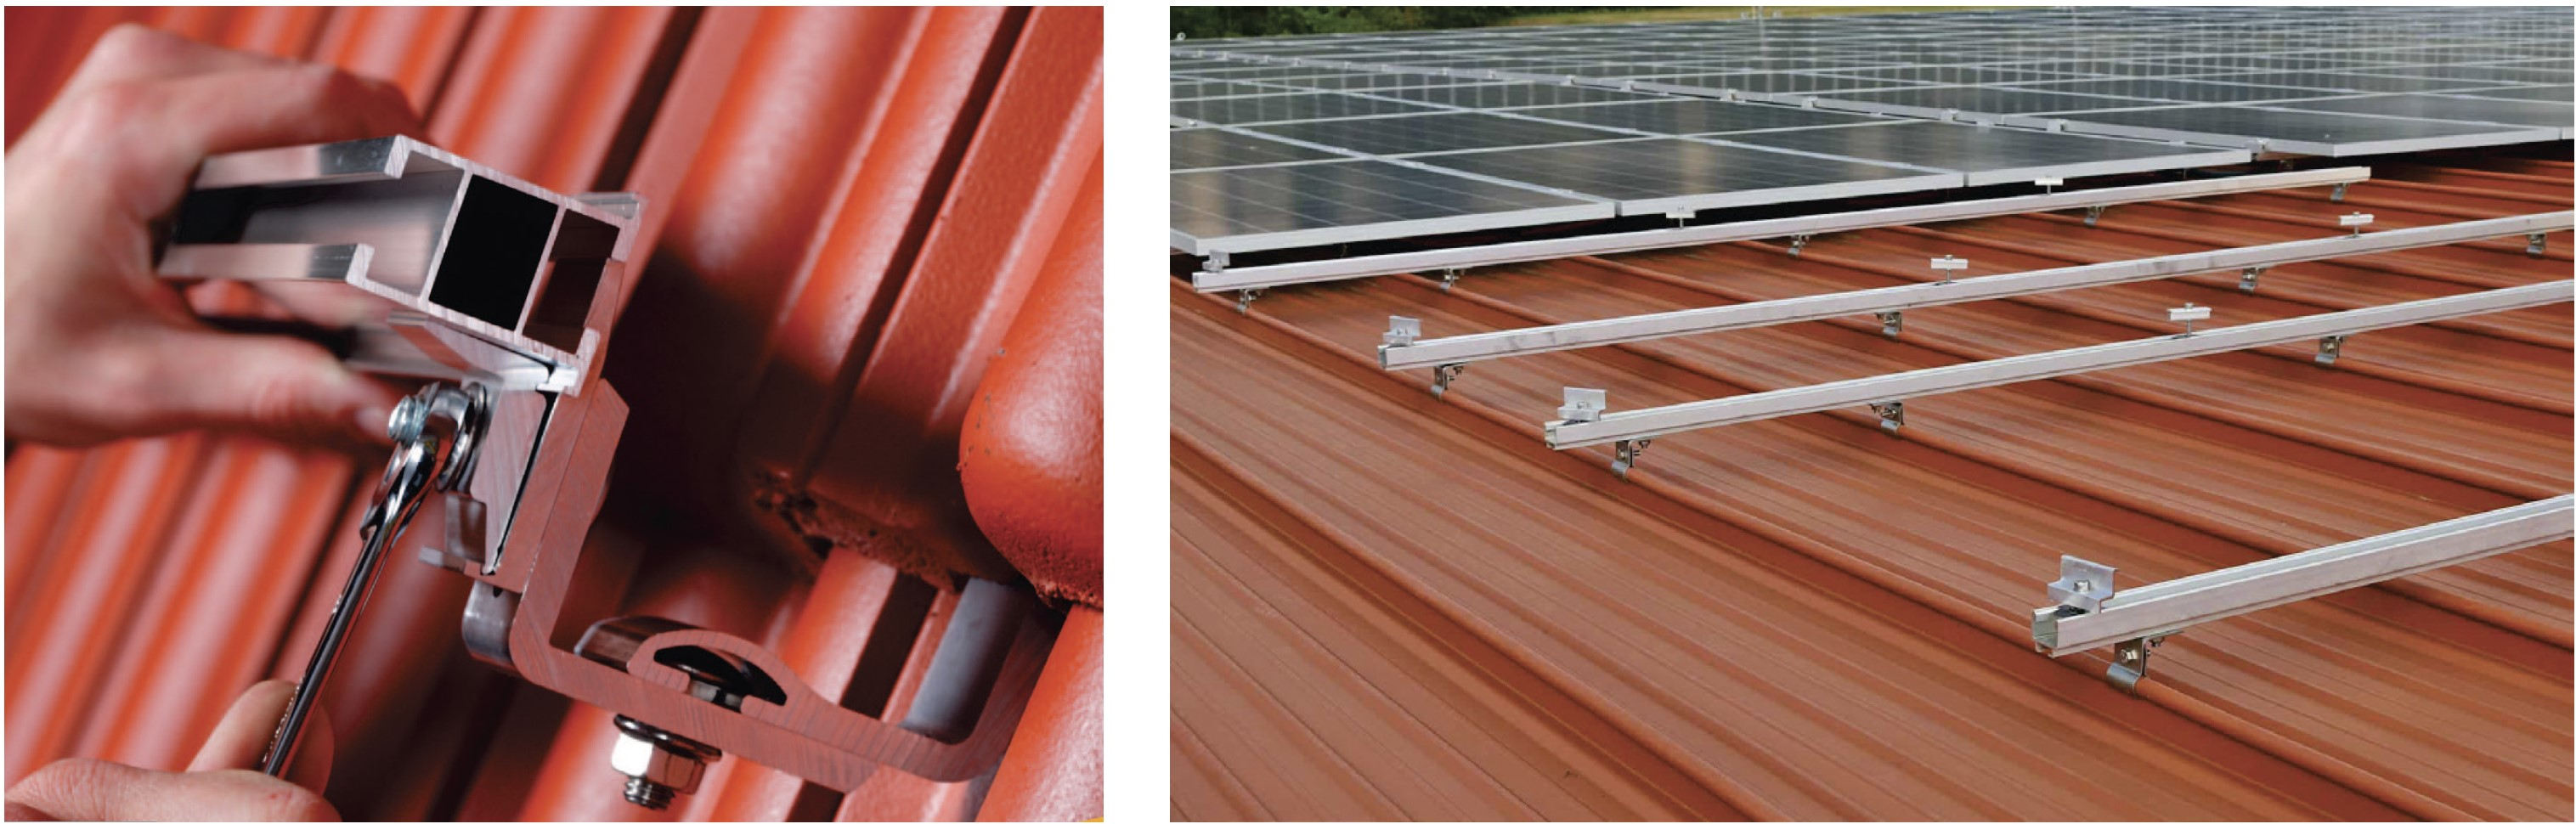
\includegraphics[width=0.85\columnwidth]{images/Einlagiges Schienensystem 2.jpg}


\subsubsection{Zweilagiges Schienensystem (Kreuzverbund)}
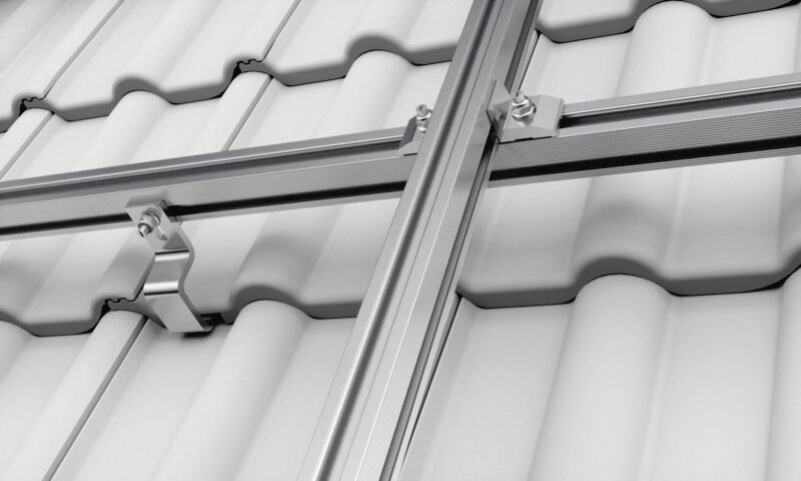
\includegraphics[width=0.48\columnwidth]{images/Zweilagiges Schienensystem (Kreuzverbund).png}



\subsection{Modulbefestigung}
\subsubsection{Modulklemmen}
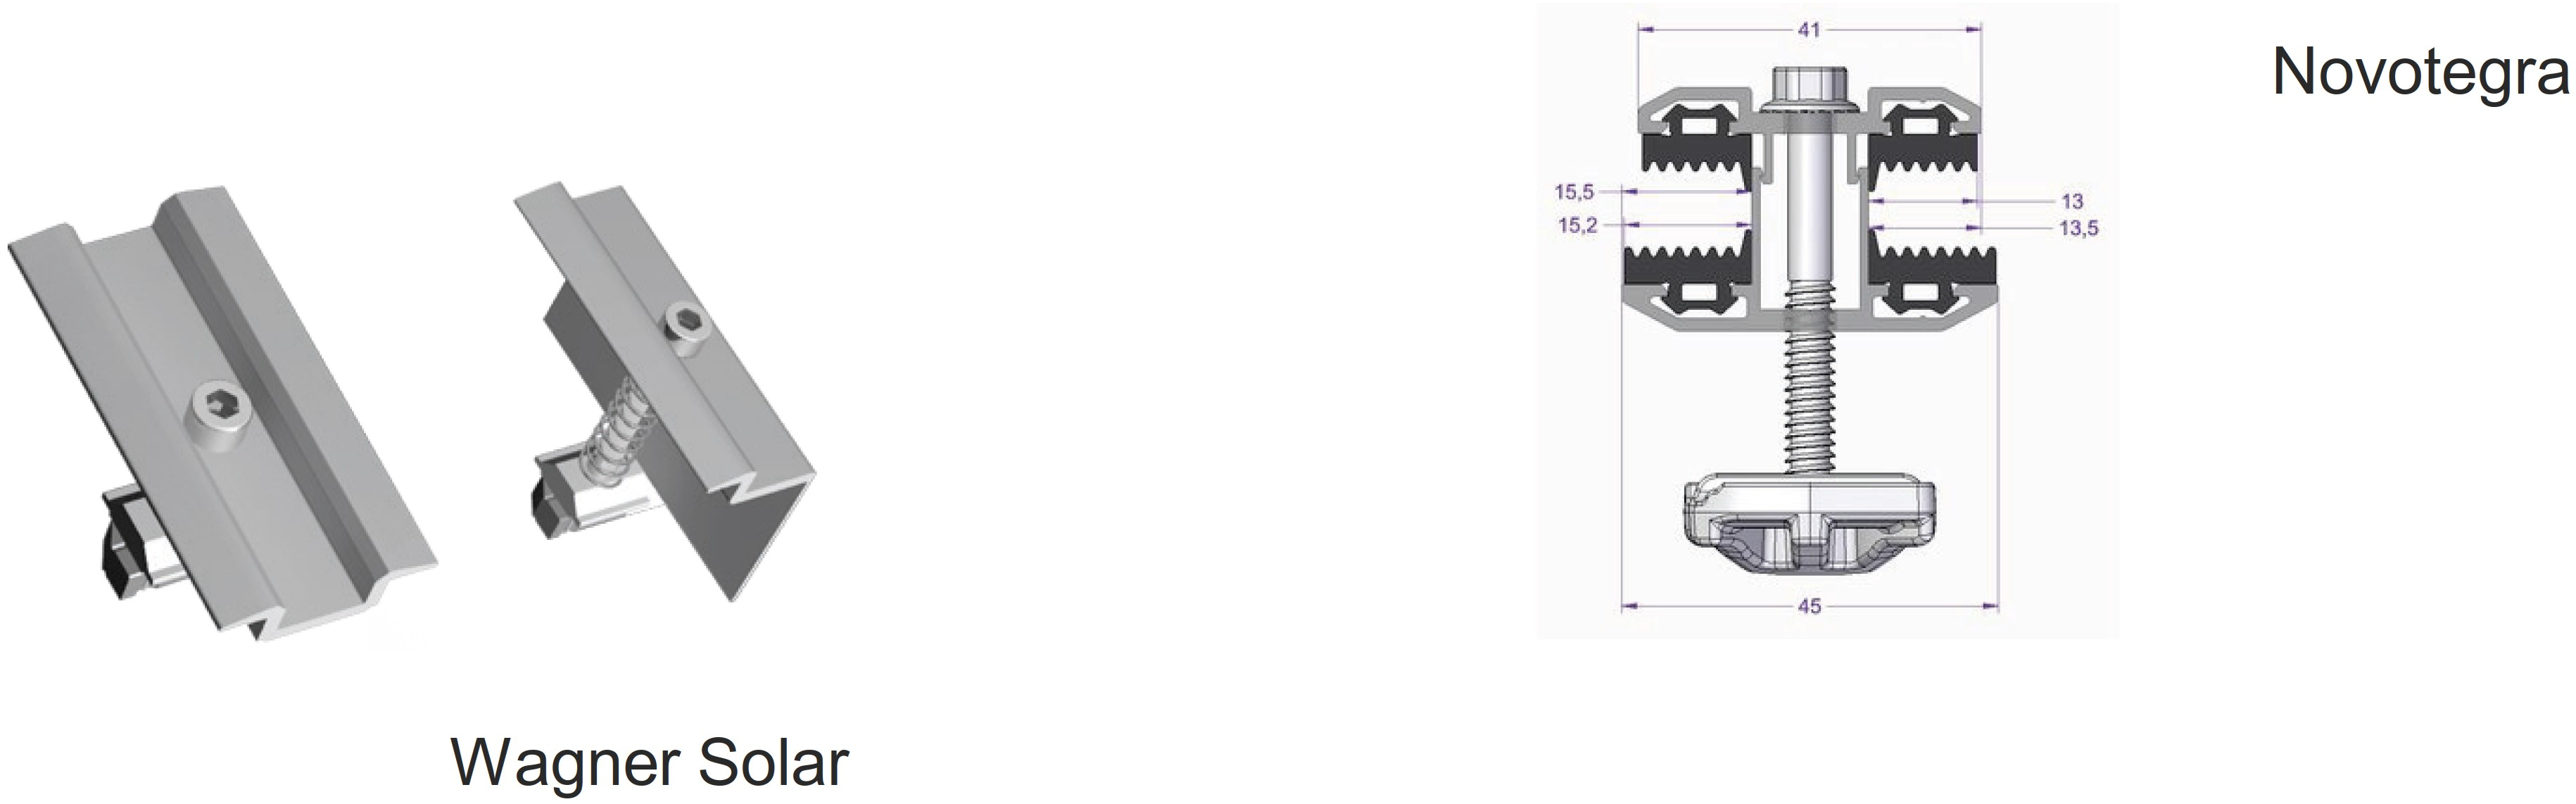
\includegraphics[width=0.95\columnwidth]{images/Modulklemmen.jpg}


\subsubsection{Einlegesystem}
\begin{minipage}[t]{0.48\columnwidth}
    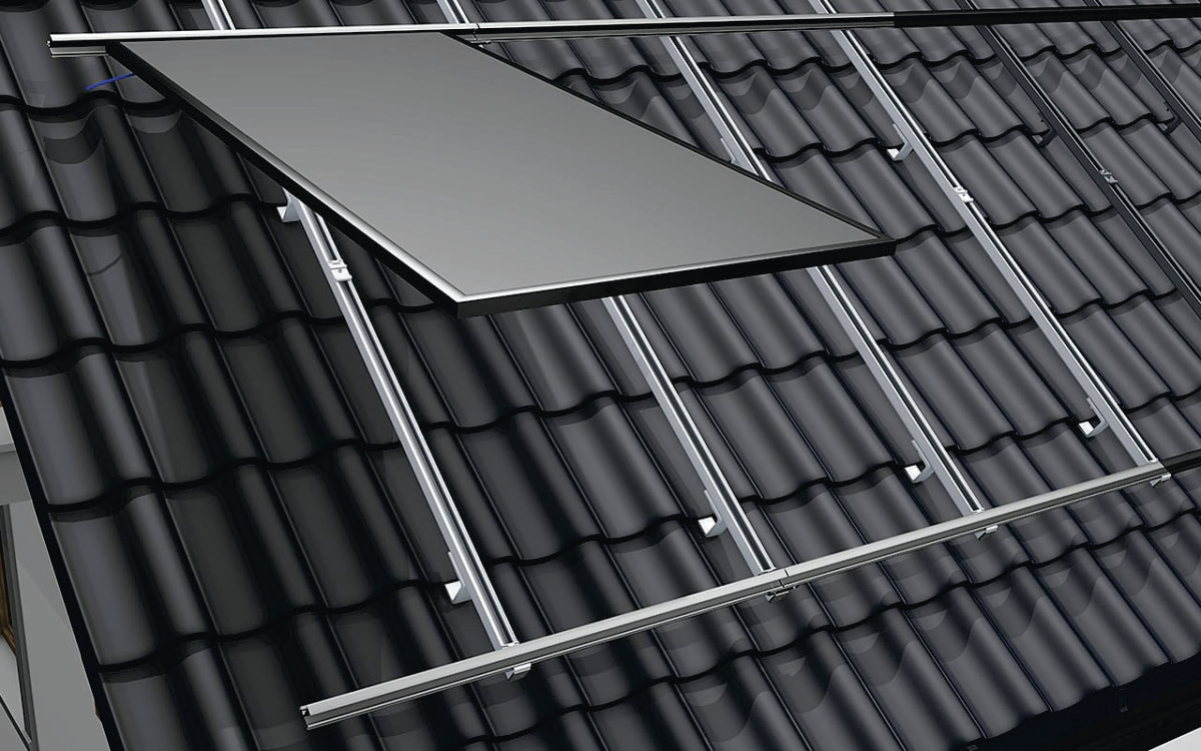
\includegraphics[width=0.95\columnwidth]{images/Einlegesystem_1.png}
\end{minipage}
\hfill
\begin{minipage}[t]{0.48\columnwidth}
    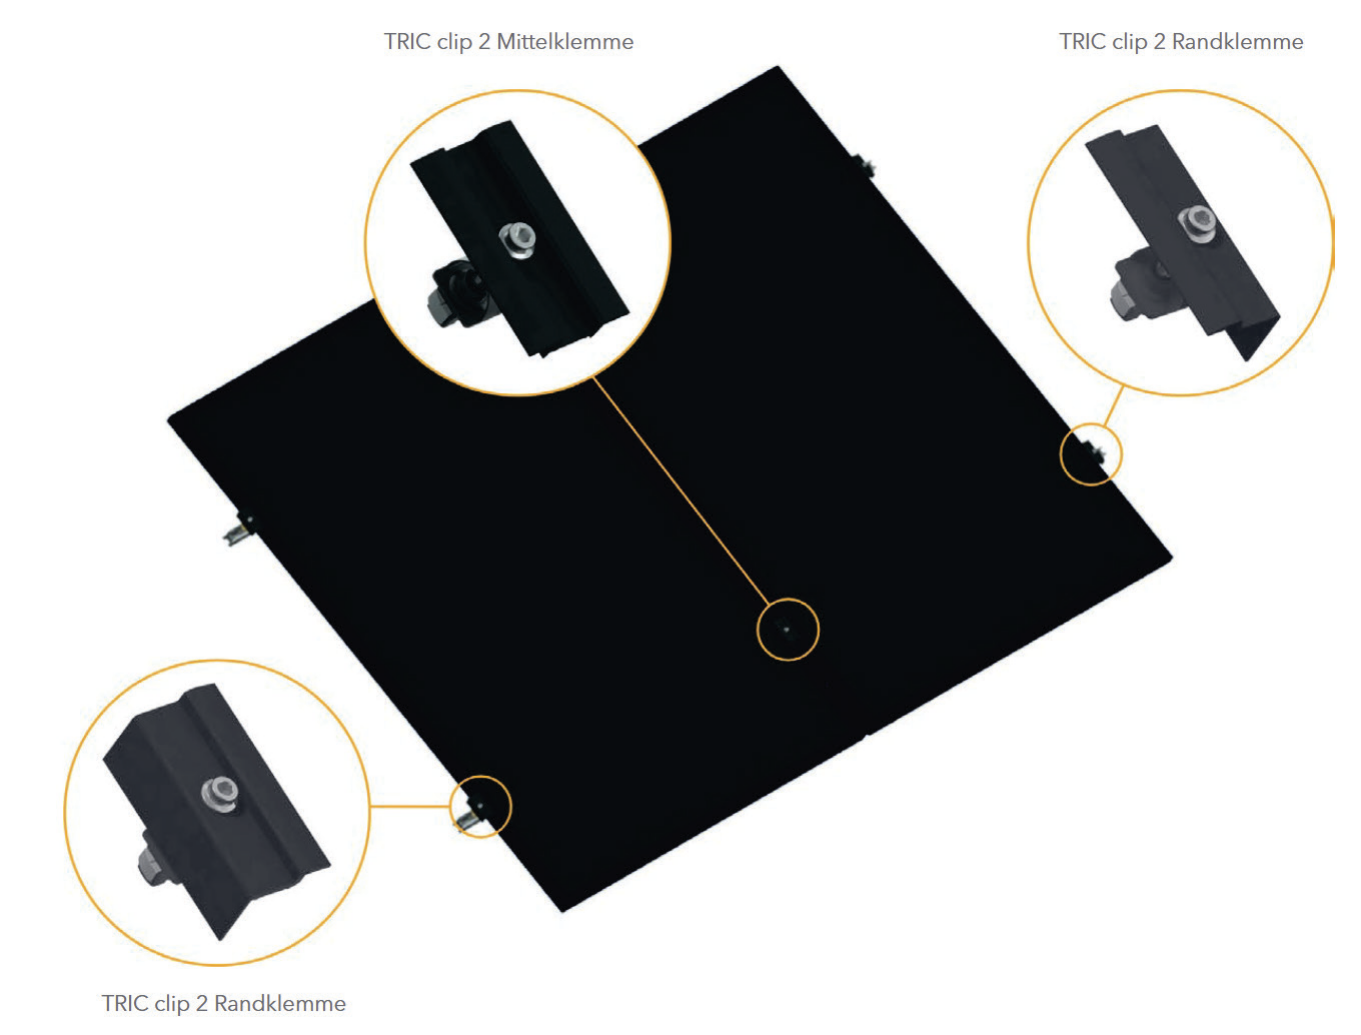
\includegraphics[width=0.95\columnwidth]{images/Einlegesystem_2.png}
\end{minipage}



\subsection{Zubehör}

\subsubsection{Kabelführung}
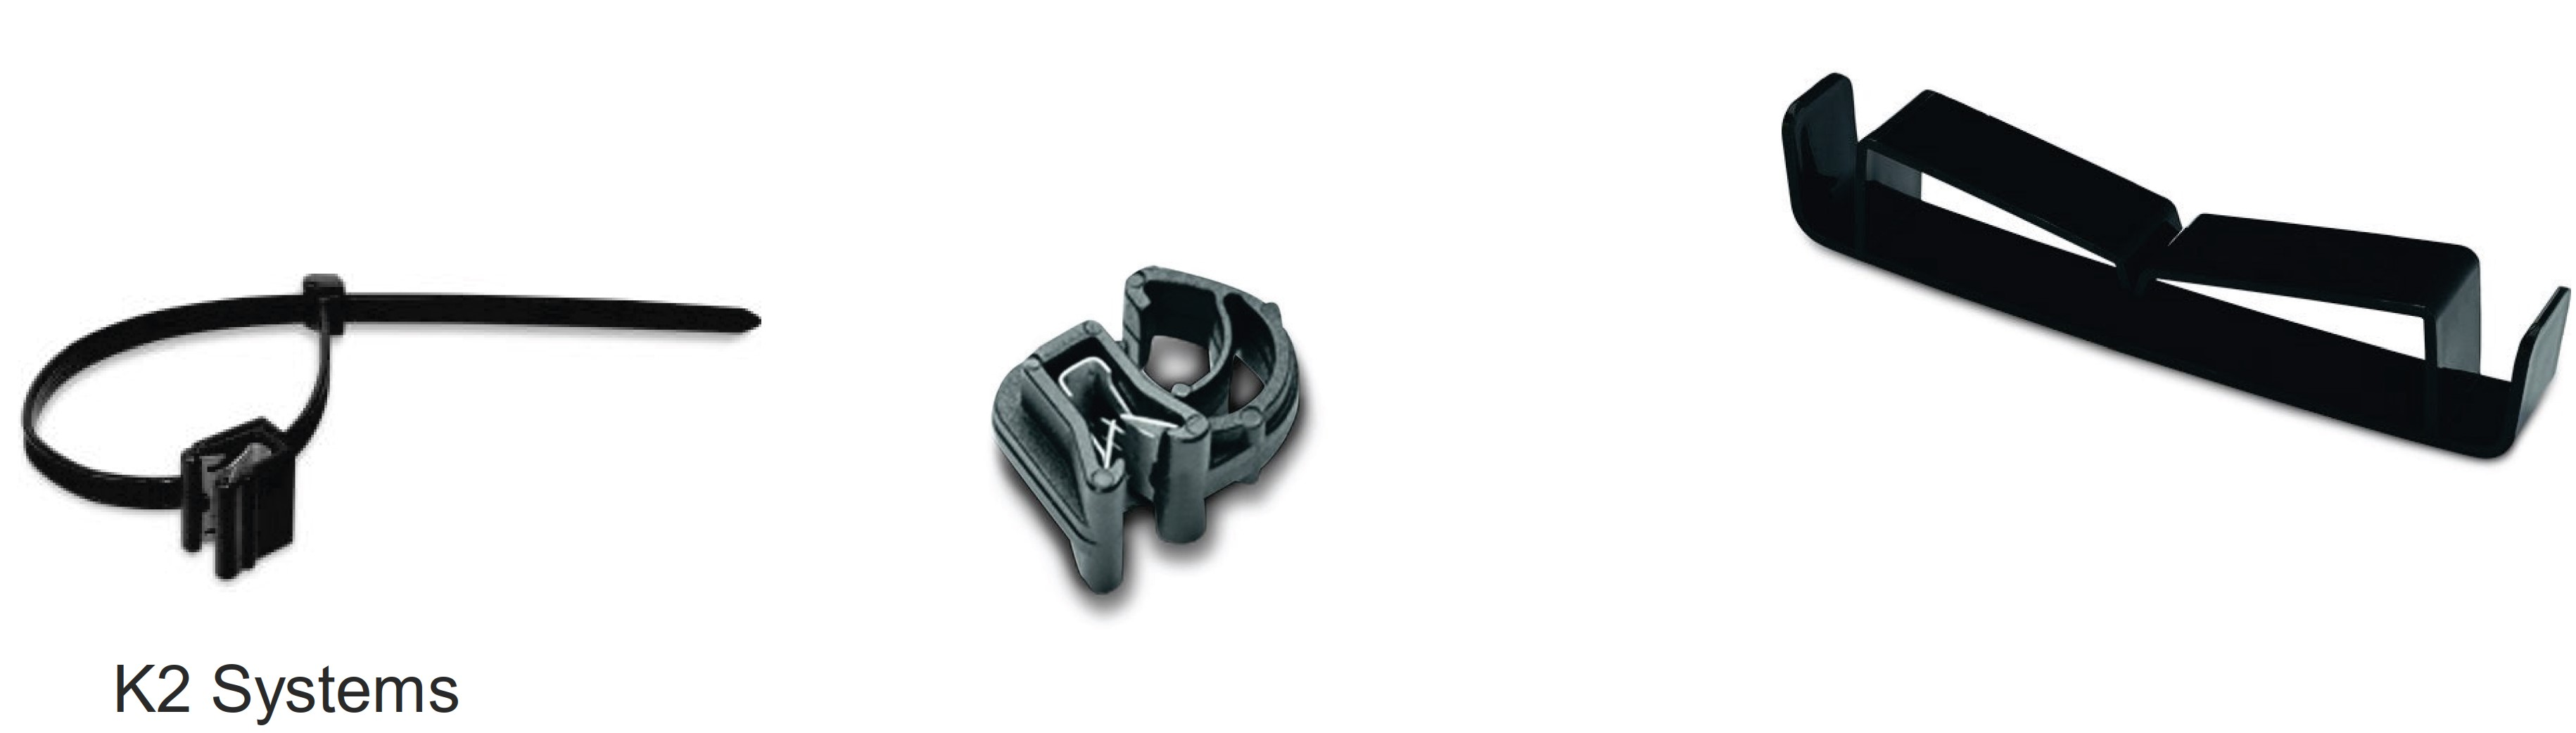
\includegraphics[width=0.95\columnwidth]{images/Kabelführung_1.jpg}\\
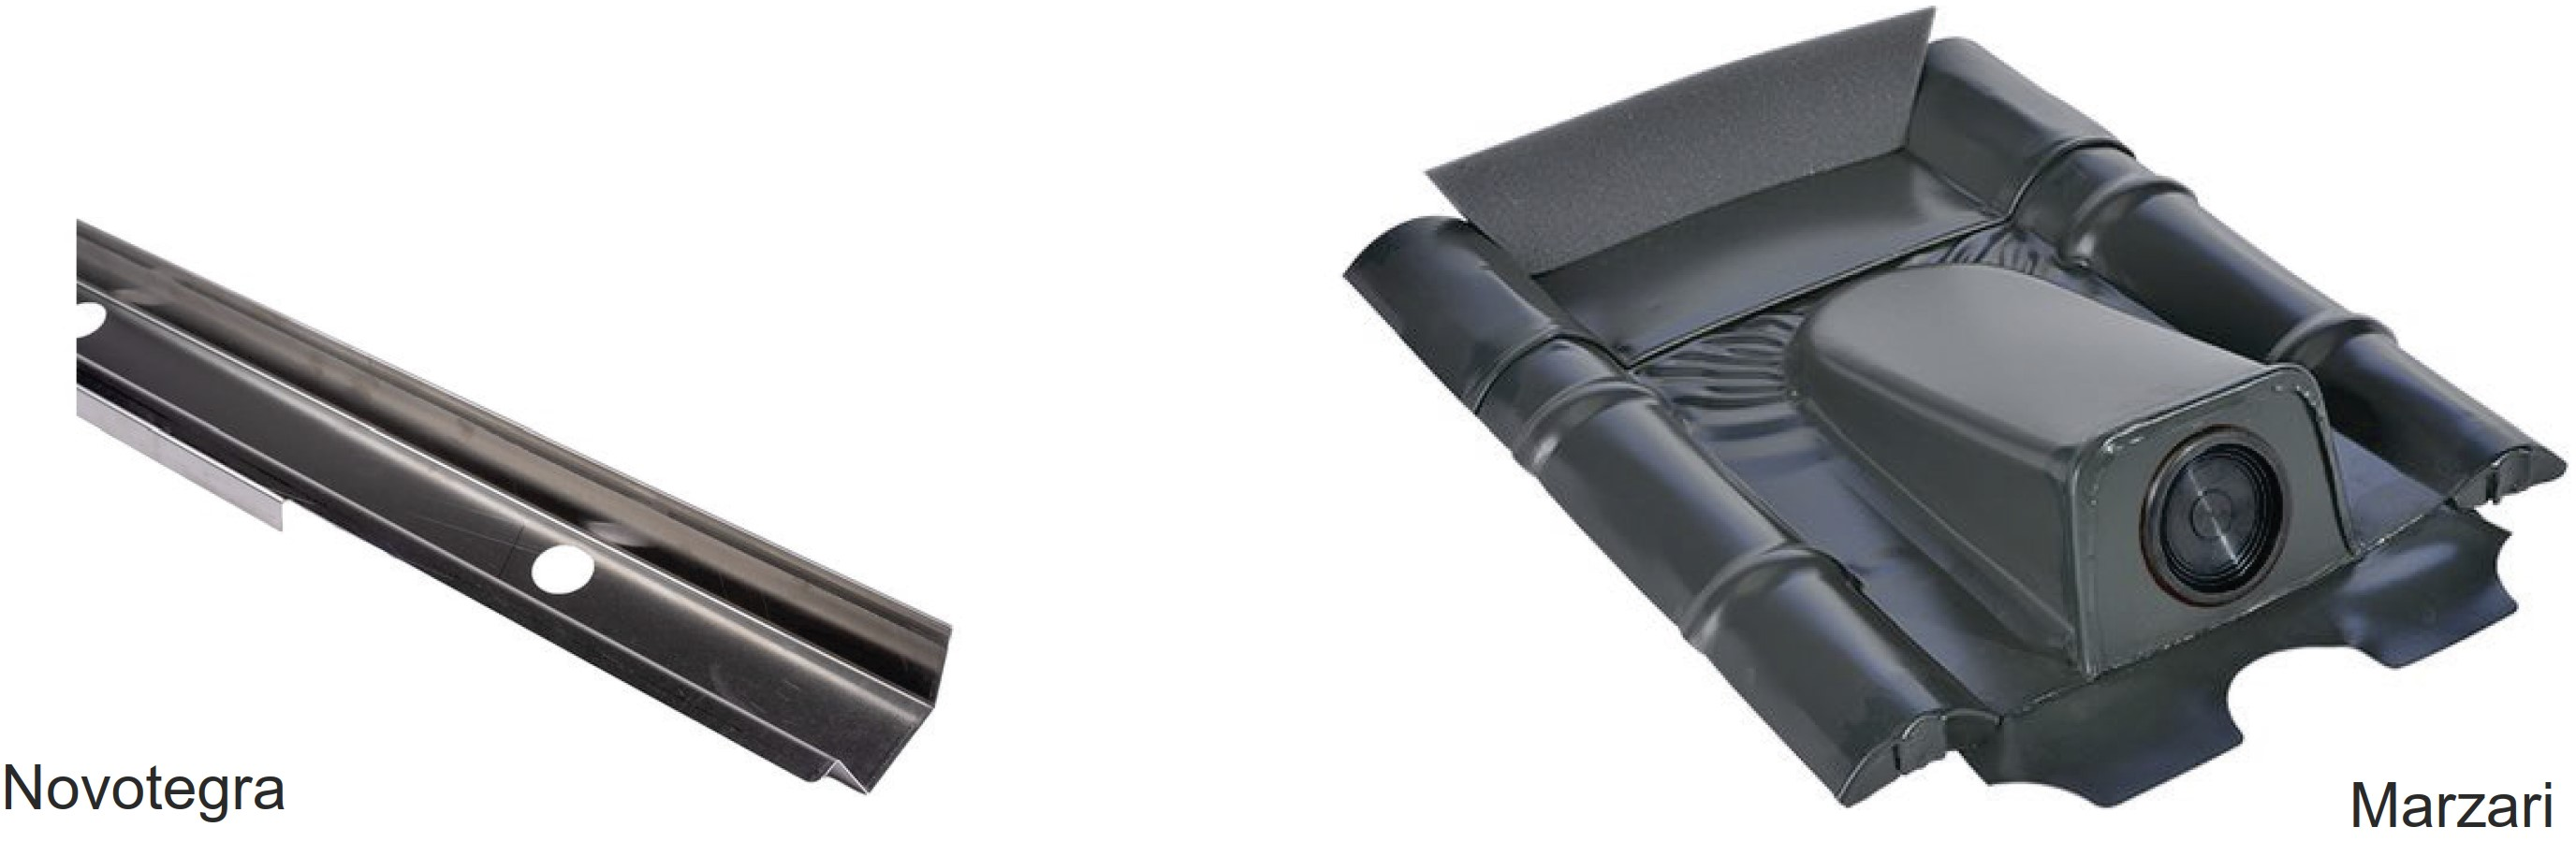
\includegraphics[width=0.95\columnwidth]{images/Kabelführung_2.jpg}


\subsubsection{Schneefang}
\begin{minipage}[t]{0.48\columnwidth}
    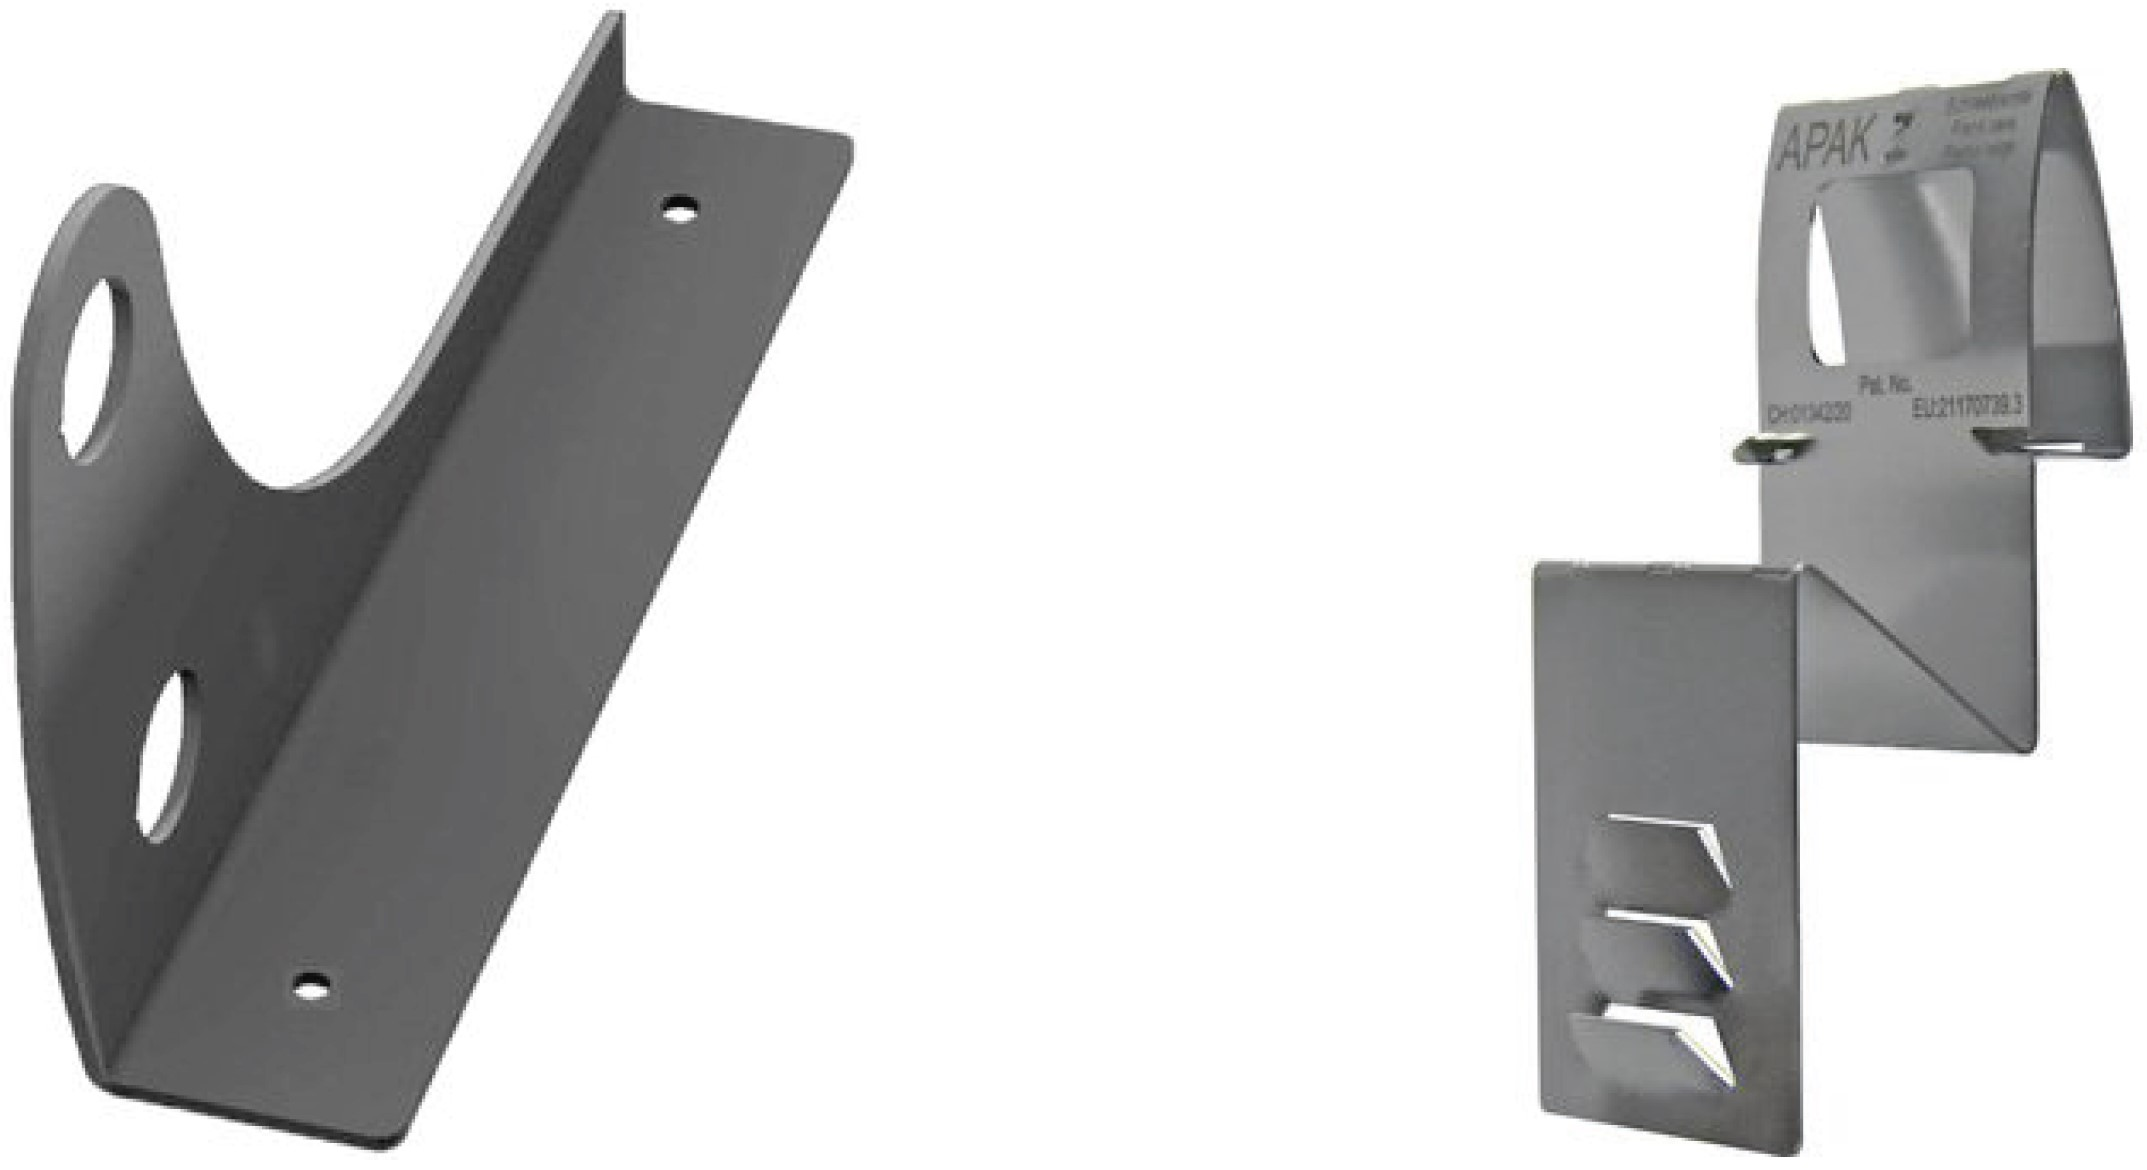
\includegraphics[width=0.95\columnwidth]{images/Schneefang_1.jpg}
\end{minipage}
\hfill
\begin{minipage}[t]{0.48\columnwidth}
    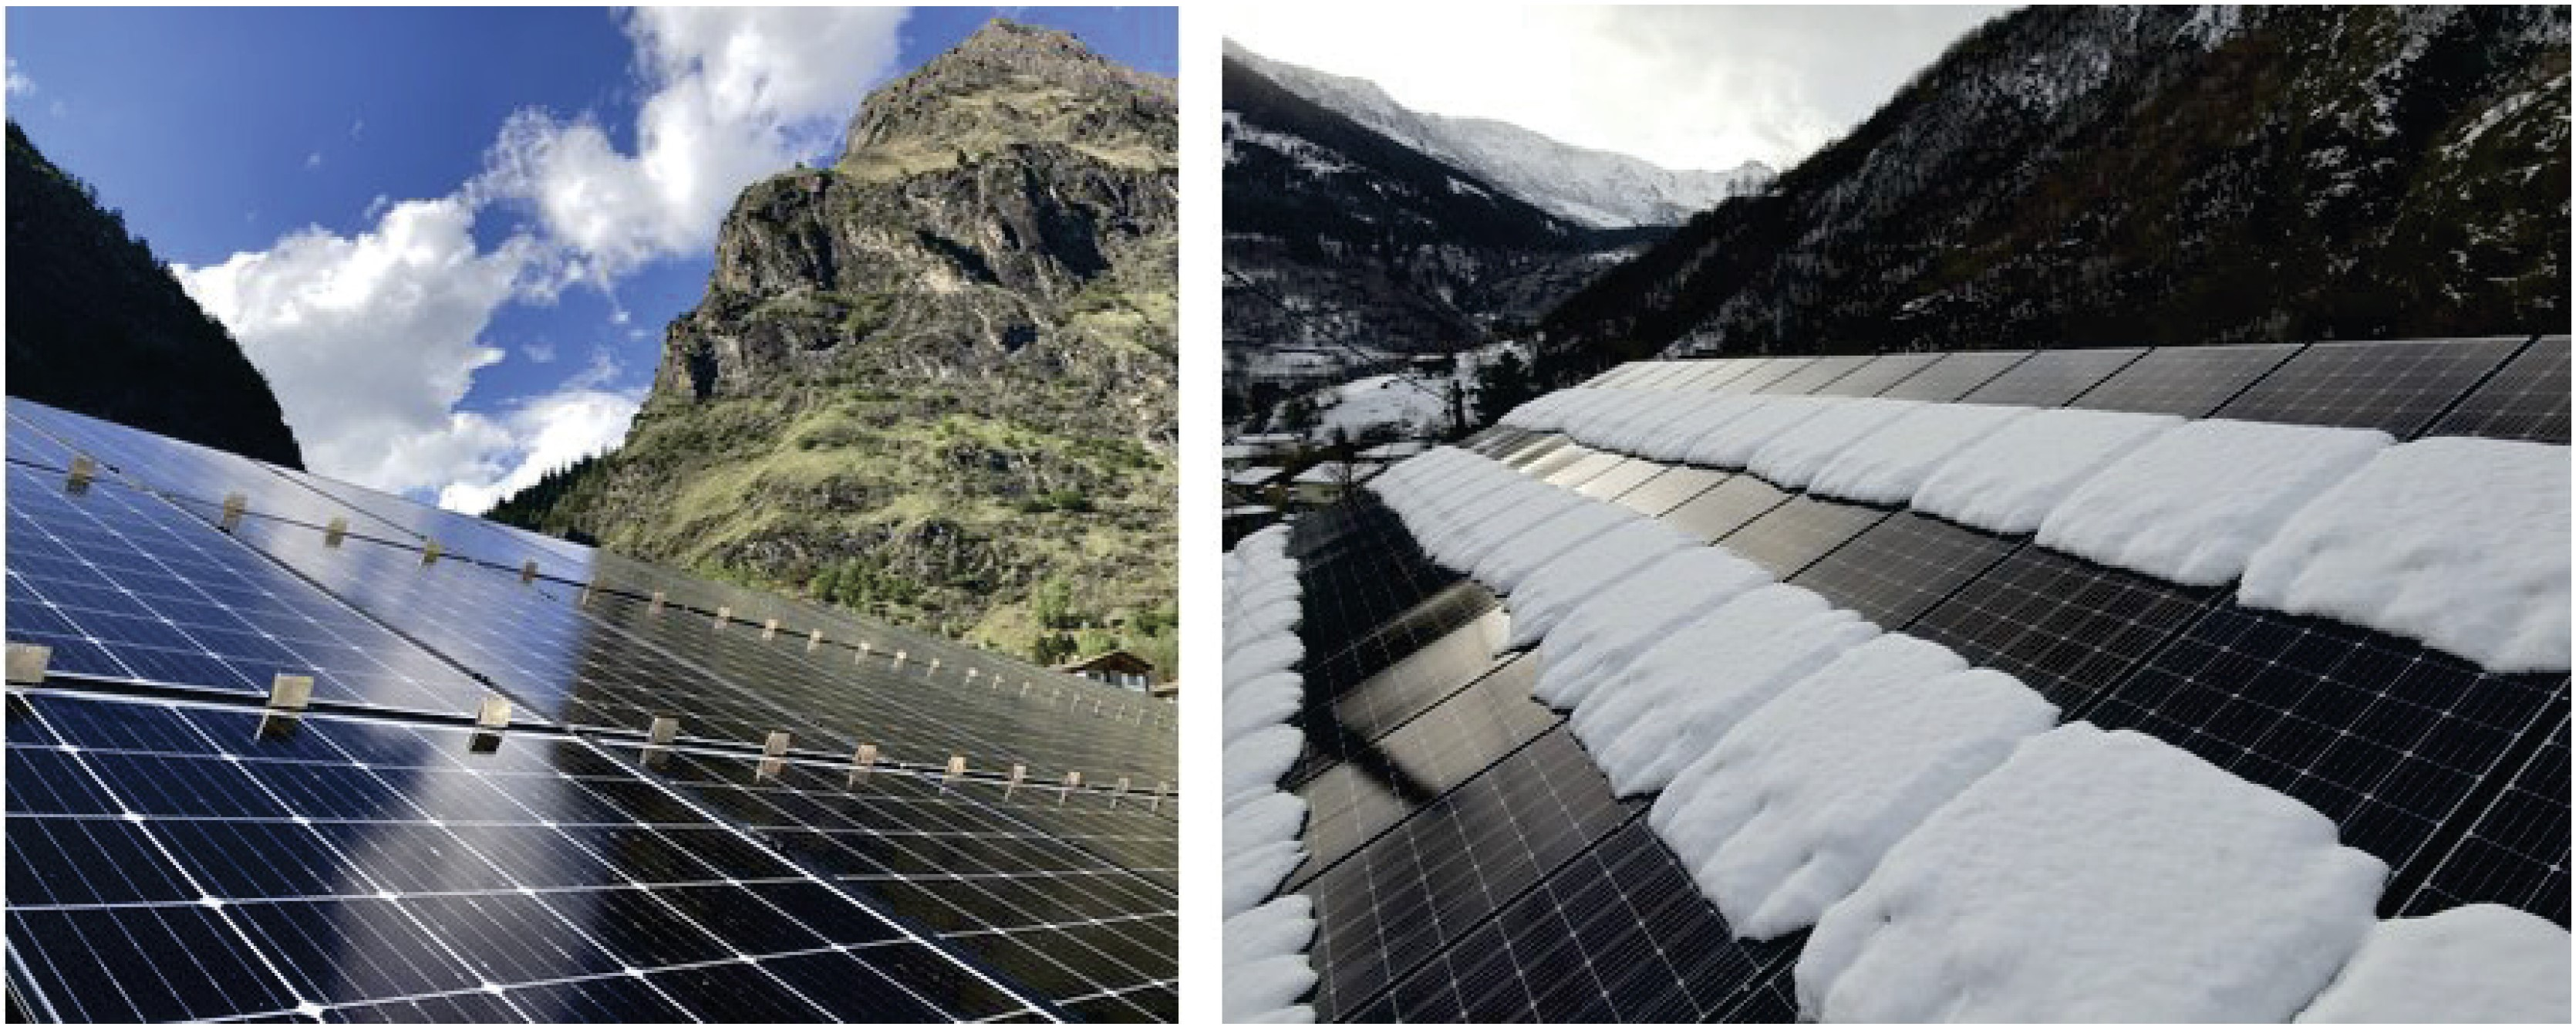
\includegraphics[width=0.95\columnwidth]{images/Schneefang_2.jpg}
\end{minipage}

%\end{comment}
\subsection{Blitzschutz und Erdung}

\begin{minipage}[c]{0.28\columnwidth}
    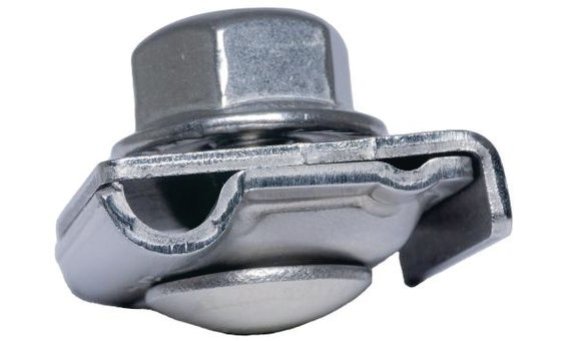
\includegraphics[width=0.95\columnwidth]{images/Blitzschutz.png}
\end{minipage}
\hfill
\begin{minipage}[c]{0.68\columnwidth}
    \textbf{Pflicht:}
        \begin{itemize}
            \item Blitzschutz vorhanden, Gebäudehöhe überragt
            \item Metallische Modulrahmen, nicht Schutzklasse II
            \item Überspannungsschutz fordert explizite Erdung
    \end{itemize}

    \textbf{Freiwillig:}
        \begin{itemize}
            \item Niedrige Gebäude, kein Blitzschutz vorhanden
            \item Module Schutzklasse II, isolierte Montage
        \end{itemize}

    \textbf{Immer beachten:}
        \begin{itemize}
            \item Lokale Netzbetreibervorgaben
        \end{itemize}
\end{minipage}



\subsection{Statik}
\subsubsection{Nachweise}
\begin{outline}
    \1 Dass das Dach die zusätzlichen Auflasten aufnehmen kann
    \1 PV-Module und Montagesystem
        \2 Grundlage: SIA 261 \glqq Einwirkungen auf Tragwerke\grqq
            \3 Berechnung der einwirkenden Wind- und Schneelasten
        \2 Windlasten
            \3 Entscheidend meistens Windsogkräfte
            \3 Unterscheidung in Dachmittel-, Rand- und Eckbereich
            \3 U.a. abhängig von Gebäudehöhe und Bodenrauigkeit
        \2 Zu berücksichtigende Schneelast insbesondere abhängig von
            \3 Dachneigung und Dachform
            \3 Höhenlage und Bezugshöhe
\end{outline}
\begin{comment}
    
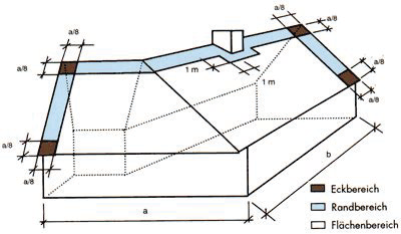
\includegraphics[width=0.75\columnwidth]{images/Statik.png}


\subsubsection{Beispiel Schneelasten}
\textbf{SIA 261 Anhang D “Bezugshöhe für Schneelasten”}\\
Bezugshöhe \(h_0\), (nicht anwendbar auf Bauwerke über 2000 m Meereshöhe)

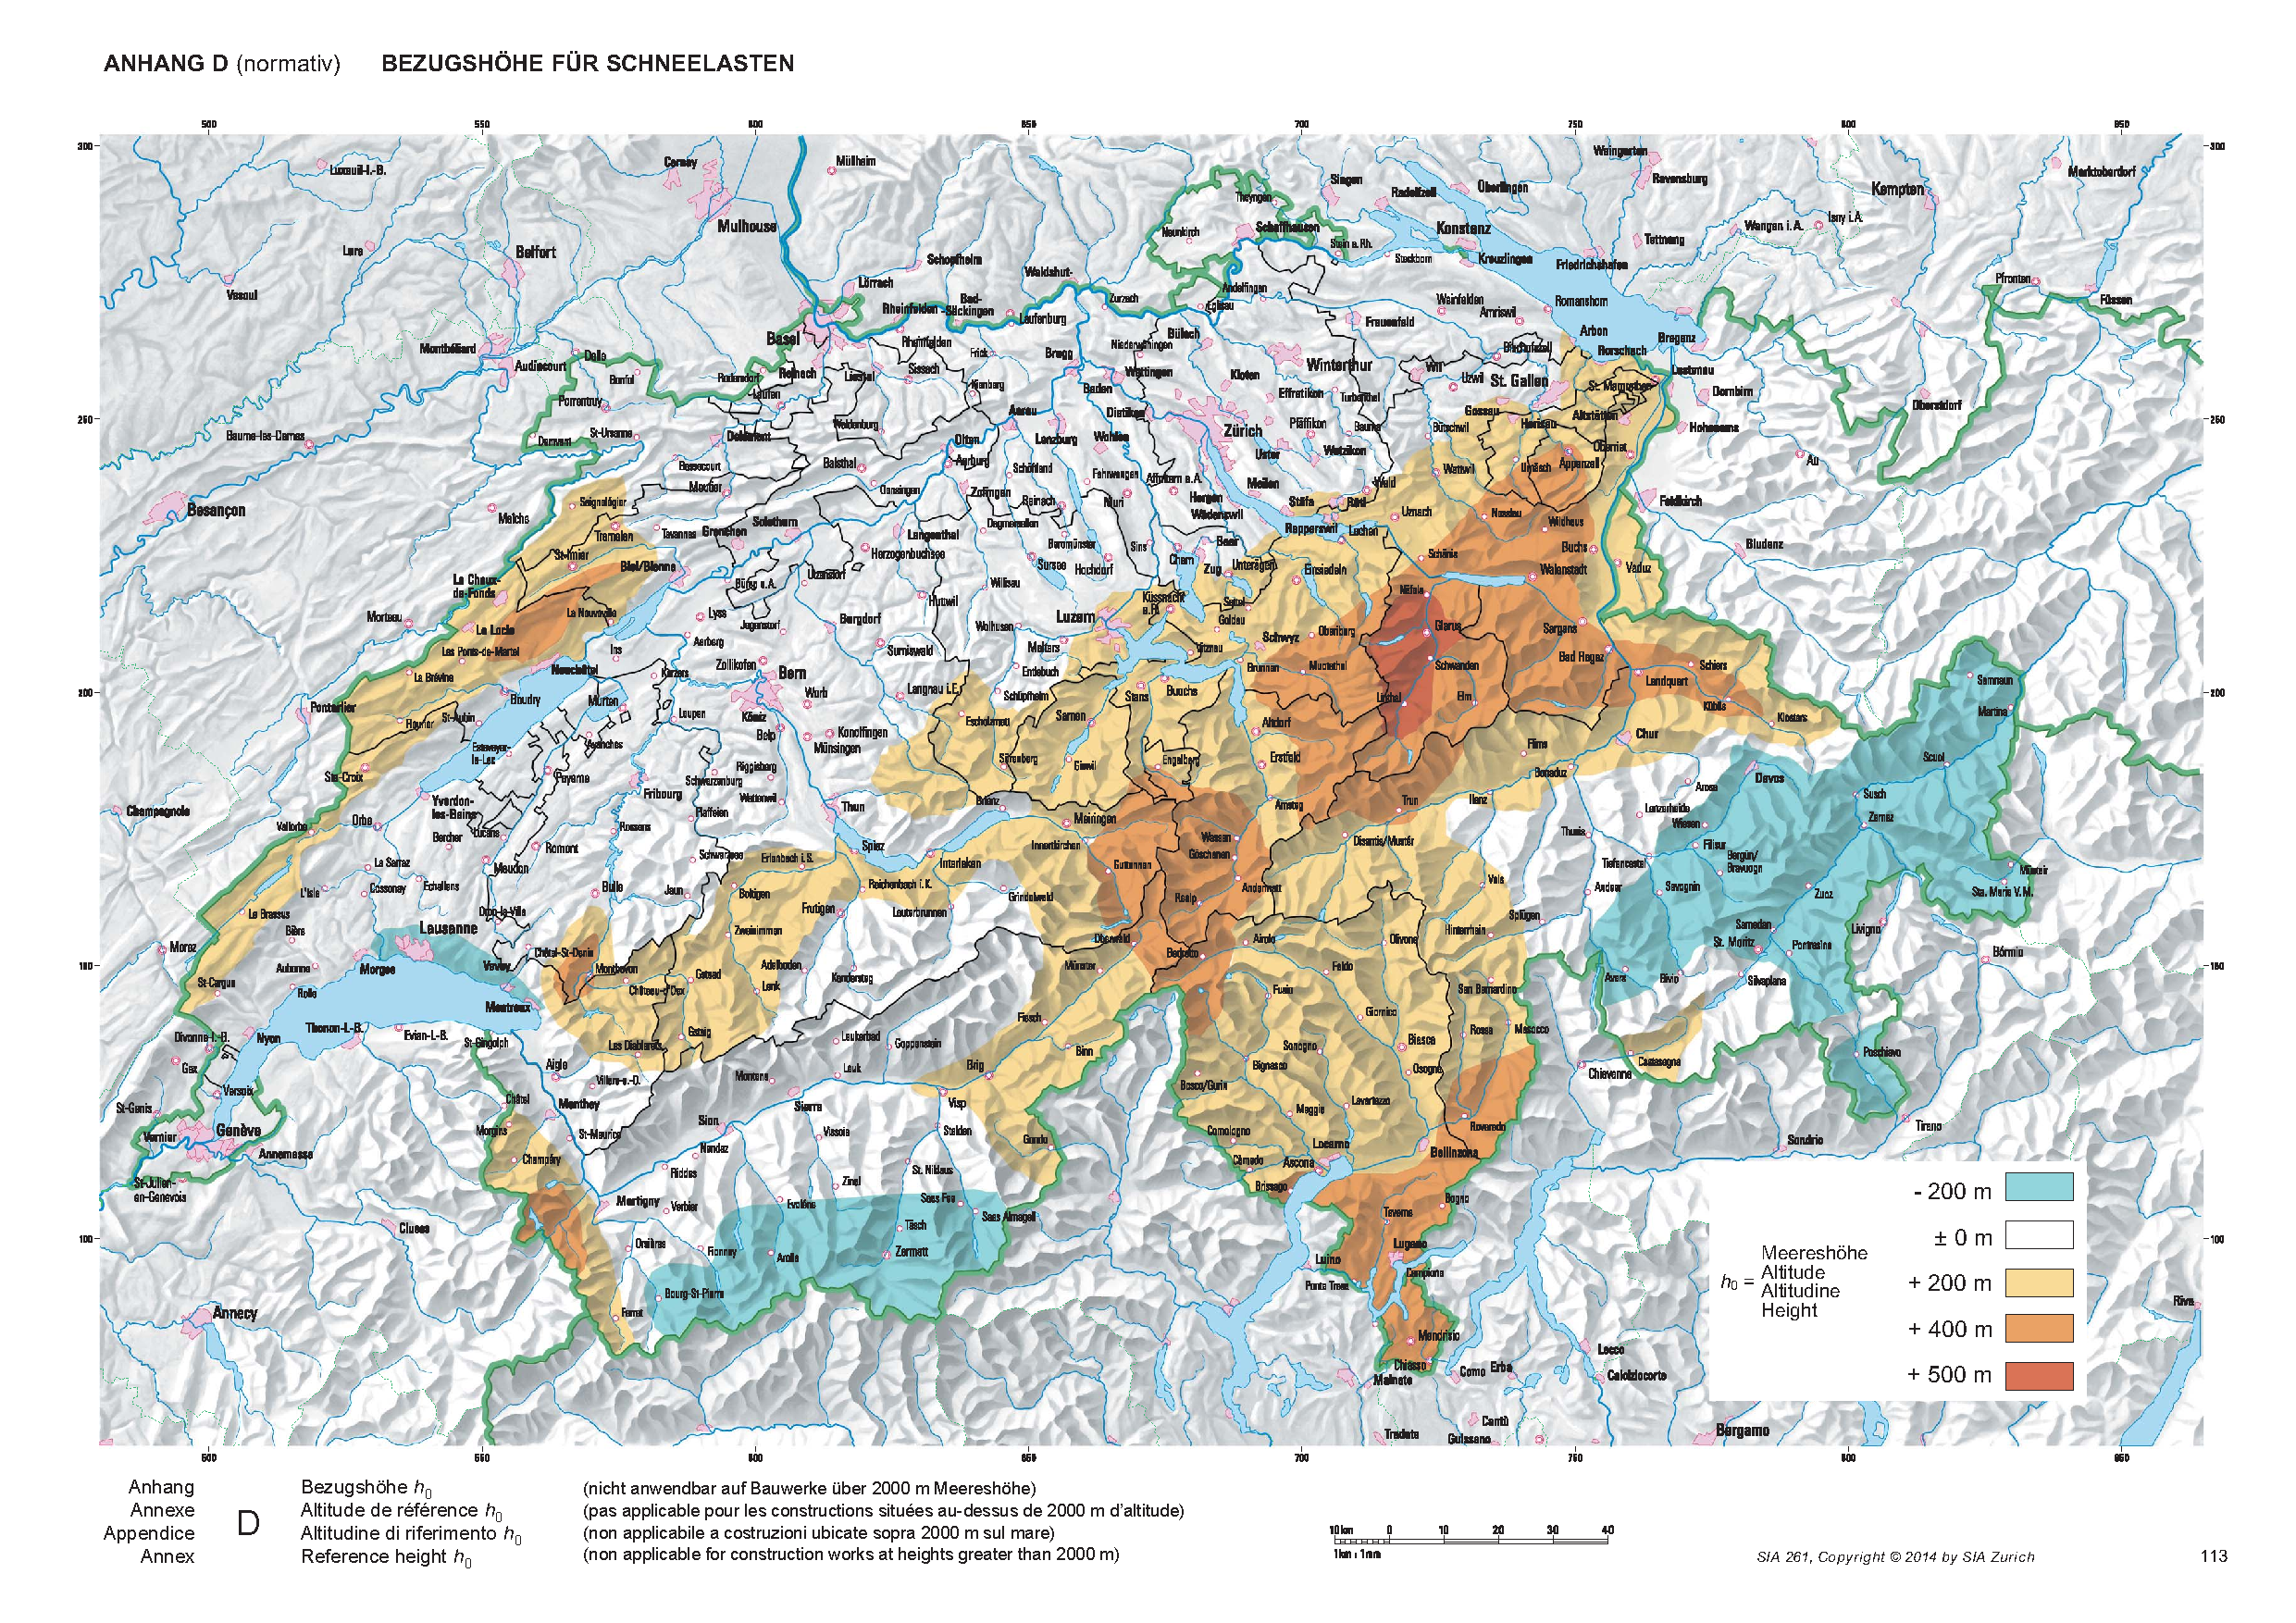
\includegraphics[width=1\columnwidth]{images/261_2014_d_Anhang_D.PDF}

\end{comment}